\documentclass{tufte-handout}\usepackage[]{graphicx}\usepackage[]{color}
%% maxwidth is the original width if it is less than linewidth
%% otherwise use linewidth (to make sure the graphics do not exceed the margin)
\makeatletter
\def\maxwidth{ %
  \ifdim\Gin@nat@width>\linewidth
    \linewidth
  \else
    \Gin@nat@width
  \fi
}
\makeatother

\definecolor{fgcolor}{rgb}{0.345, 0.345, 0.345}
\newcommand{\hlnum}[1]{\textcolor[rgb]{0.686,0.059,0.569}{#1}}%
\newcommand{\hlstr}[1]{\textcolor[rgb]{0.192,0.494,0.8}{#1}}%
\newcommand{\hlcom}[1]{\textcolor[rgb]{0.678,0.584,0.686}{\textit{#1}}}%
\newcommand{\hlopt}[1]{\textcolor[rgb]{0,0,0}{#1}}%
\newcommand{\hlstd}[1]{\textcolor[rgb]{0.345,0.345,0.345}{#1}}%
\newcommand{\hlkwa}[1]{\textcolor[rgb]{0.161,0.373,0.58}{\textbf{#1}}}%
\newcommand{\hlkwb}[1]{\textcolor[rgb]{0.69,0.353,0.396}{#1}}%
\newcommand{\hlkwc}[1]{\textcolor[rgb]{0.333,0.667,0.333}{#1}}%
\newcommand{\hlkwd}[1]{\textcolor[rgb]{0.737,0.353,0.396}{\textbf{#1}}}%

\usepackage{framed}
\makeatletter
\newenvironment{kframe}{%
 \def\at@end@of@kframe{}%
 \ifinner\ifhmode%
  \def\at@end@of@kframe{\end{minipage}}%
  \begin{minipage}{\columnwidth}%
 \fi\fi%
 \def\FrameCommand##1{\hskip\@totalleftmargin \hskip-\fboxsep
 \colorbox{shadecolor}{##1}\hskip-\fboxsep
     % There is no \\@totalrightmargin, so:
     \hskip-\linewidth \hskip-\@totalleftmargin \hskip\columnwidth}%
 \MakeFramed {\advance\hsize-\width
   \@totalleftmargin\z@ \linewidth\hsize
   \@setminipage}}%
 {\par\unskip\endMakeFramed%
 \at@end@of@kframe}
\makeatother

\definecolor{shadecolor}{rgb}{.97, .97, .97}
\definecolor{messagecolor}{rgb}{0, 0, 0}
\definecolor{warningcolor}{rgb}{1, 0, 1}
\definecolor{errorcolor}{rgb}{1, 0, 0}
\newenvironment{knitrout}{}{} % an empty environment to be redefined in TeX

\usepackage{alltt}
\usepackage{hyperref}

\title{How can the Santa Ana sucker be saved?}
\author{Marc Los Huertos}
\IfFileExists{upquote.sty}{\usepackage{upquote}}{}
\begin{document}

\maketitle

\section{Introduction}

According to Kolbert 2015, we are in the midst of a dramatic extinction event that is rivaling major catastrophic extinctions in the past. The difference with the current situation is the cause: The dominance of human beings over the Earth's surface had led to the extirpation of thousands of species, and counting. 

It's easy to second guess various scientific and policy questions with respect to endangered species, but when we begin to evaluate a specific taxon, we quickly learn that we are not just in an ecological web, but our policy and regulatory processes are embedded in a complex context of land use history and economic agendas. Thus, for this project, we shall focus on the Santa Ana sucker (\emph{Catostomus santaanae}) of an extinction potential.  

\begin{figure}
    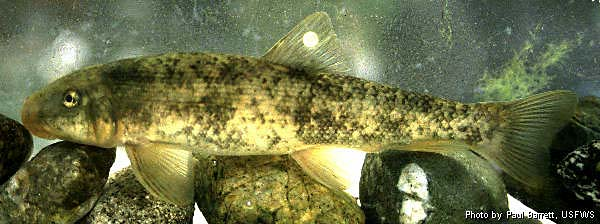
\includegraphics[width=1.0\textwidth]{Catostomus_santaanae.jpg}
  \caption{Santa Ana sucker, \emph{Catostomus santaanae} is a member of the sucker family (Catostomidae) and endemic to California.}
\end{figure}

\subsection{Driving Question}

This project will attempt to answer the following question, "How can we save the Santa Ana sucker?" As we have seen, this type of generic question needs to be constrained, defined, and subject to what we already know or will learn about the topic. In addition, we need to define the terms used in the question, such as who is "we"? What do we mean by "save"?  And finally, when we ask "how", what are the options available that might fit into the "how"? 

\section{Learning Goals}

In the broadest sense, we will learn how to conduct a scientific study to meet policy and regulatory goals -- in this case for the Endangered Species Act. By selecting the Santa Ana sucker, we have "constrained" the methodological options available, largely to aquatic sciences, such as hydrology, geomorphology, biogeochemistry, ecology, and animal behavior. As such, we will specific skills: 

\begin{itemize}
  \item To evaluate sucker habitat using the following tools:
  \begin{itemize}
    \item Define water quality goals;
    \item Characterize hydrology and geomorphology habitat; and
    \item Analyze community profile of periphyton.
  \end{itemize}
  \item To propose and compare options to improve Santa Ana sucker habitat.
  \item To prepare sets of practical and effective measures that might protect (or increase) the extant populations of the Santa Ana sucker.
\end{itemize}

\subsection{Why these learning goals?}

Scientific methods vary dramatically accross and within disciplines and subdisciplines, so no course can cover even a fraction of scientific methods available. We have picked the methods above because they might provide the tools to consider how to protect and restore Santa Ana sucker populations.

\section{Project Stages}

\begin{itemize}
  \item Session 1: Welcome to the Santa Ana River (August 30/31)
  \item Session 2: Define \textbf{Public Product} (September 6)  
  \item Session 3: Revise \textbf{Driving Question}, list resources needed,  \& develop \textbf{Team Contract} (Sept. 6/7)
  \item Session 4: Read, clarify, or develop appropriate \textbf{SOPs} (Sept 6-12)
  \item Session 5: \textbf{Field Work} (Sept 13/14)\sidenote{Kai wants us out on the 5th of Sept. We will see what we can do.}
  \item Session 5: \textbf{Data Analysis} (September 20/21)
  \item Session 7: Development of \textbf{Public Products} (September 27/28)
  \item Session 6: \textbf{Presentation} of Public Products (Oct 4/5)
\end{itemize}

\section{Defining the Public Product}

The stakeholder group has defined the following products for our work:

\begin{description}
  \item[Annotated Bibliography] We shall collate, organize, and summarize scientific resources that can be digested by a range of stakeholders to help "answer" the driving question. 
  \item[Analysis of how invasive red algae affect fish behavior] Using several videography, we will capture fish behavior associated with various habitats within several reaches of the Santa Ana River.
  \item[Research Briefs] These briefs will describe the knowledge base, information gaps, and research needs for a range of topics. Each student will contribute one science brief that describes the knowledge available to "restore and protect" the Santa Ana Sucker. Each research brief, will address a different scientific issues associated with the Santa Ana sucker--where each issue addresses a specific driving question with respect to the sucker. EA 30 Research Briefs are short (3-4 pages) descriptions of recently EA30 project results. These ``briefs'' highlights also include one image, a caption (50 words), and several publication citations. Each student will develop one to several briefs that will be made available to the public.
  
Each brief will include 5 sections:

\begin{itemize}
  \item Problem definition
  \item Evidence of problem
  \item Scientific knowledge to address the problem
%  \item Description of Potential Alternative Solutions
  \item Information gaps
  \item Next Steps (which could be translated by stakeholders as potential research needs)
\end{itemize}

  \item[Presentation to HPC on findings] And as the topics develop, we will bundle briefs to produce 3-5 reports that will be made public as part of a presentation to the HPC group.
\end{description}

\subsection{Project Partners and Evaluation Criteria of Public Product}

Although the audience is the public at large, we will use several collaborators to help us define, refine, and evaluate our public products.  
Our collaborators are members of the Santa Ana sucker HPC (Habitat Planning Committe) and others parties and include: 

\begin{itemize}
  \item USFWS
  \item RCD of SB?
  \item San Bernardino Water Management Agency
  \item UC Riverside
  \item XX Consulting
\end{itemize}


%west fork...Edison... consulting report?
%Justin...

%baskin...(old Alzheimer..)

%annotate bibl. documents.

%recovery permit...

%coordinator 10A1A permit...

%6-25 980? in Carlsbad...

Working with stakeholders is a key component doing environmental science, which might be contrasted with regular scientific research. Although some make the distinction between applied and pure science, I don't find the divide all that useful. Better that getting into the morass of these definitions, let's move on to figure out what skills we need to apply while working with stakeholders. 

As it turns out, few stakeholders can really define their project until after it is complete -- much to the surprise of the both the stakeholder and the group doing the work. This is not a limitation of the stakeholders, it's that developing realistic goals with collaborators requires some investment to appreciate the resources and trust the how the product will be developed. 

There is no secret to get around this problem and even if you identify and try to work through it, you might still find that the project doesn't meet the ``expectations'' of the stakeholder -- which were either unrealistic or poorly defined or both. Alternatively, it's easy for a collaborator to promise too much or to fail to appreciate the complexity of a project until it's too late. 

\begin{description}
  \item[Active Listening] Careful listening and echoing what stakeholders say is an extremely important to develop a successful partnership with stakeholders. Asking for clarity and follow up questions will help you define what the goals of the project in collaboration.
  \item[Defining Success] As a key component of collaboration is ensuring that all parties agree on what success look like. For example, this would include examples of ``models'' to emulate or avoid. In addition, going through the project will help articulate clear expectations about the public product and the workload to get there.
  \item[Outlining a Process] The process can also be called, ``project management'', which sounds a bit stale. However, project management is a key aspect of working with stakeholders so each party appreciates the how milestones are met and contribute the the final project. 
  \item[Professionalism and Completion] Part of professionalism is meeting the stakeholder expecation --- but it's more. Sure, it often entails that the product is completed on time and that it meets and exceeds expectations. But it also means that when asked if they would hire you again, they would answer 'yes without hesitation.'  Please keep this in mind, at every stage of the process.  
\end{description}

\begin{marginfigure}
   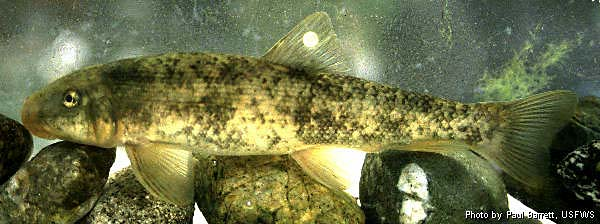
\includegraphics[width=1.0\textwidth]{Catostomus_santaanae.jpg}
  \caption{The Santa Ana sucker \emph{Catostomus santaanae}.}
\end{marginfigure}

During the summer, our research partners describe various interests they had with our class. Below are some of the opinions expressed:

\begin{description}
  \item[Kai Pelenscar]US Fish and Wildlife Service
  \begin{quote}
Based on the current data set we have on sucker biology and habitat preference, I would like to identify data gaps where student work would contribute to species' conservation as well as contribute to research or other types of projects. In order to prioritize a list of data gaps, I need to know where we stand on the ongoing research projects relating to sucker.

Also, instead of tying the change in habitat to a shutdown, potentially a high velocity flushing flow from RIX [Water treatment facility] would provide data for a measure proposed by Heather's group. 

\noindent Note on 8/29

I really do see value in getting videography data for sucker. Maybe even two cameras placed in opposing sides of the same pool. Do you know if the camera would be effected by electroshock? I would think the waterproof housing would effectively insulate against shock damage. Right? 

You could look at pre, during and post sampling of a reach to assess habitat usage (pre versus post sampling, red alga versus native/diatoms), habitat disturbance from the sampling, and qualitative assess the effect of the sampling on the fish (change in fish numbers, behavioral changes, etc.). Three sampling methods will be employed in the same area, one after the other. Another assessment could be done looking at differences between the three sampling methods (snorkeling, seining, electroshocking). There is a time lag between sampling methods. Not sure if this would be enough time for fish behavior to return to normal. Nonetheless, these data would better inform the biology and behavior of the species and may be informative to measures the Service creates to minimize impacts to the species. 

If the data looks to be high quality after the first round you could repeat one or more additional times throughout the native fishes survey in similar or different habitat types. Security of your hardware would be ensured as the sampling would coincide with the fish survey. This work would inform future projects that could employ in-stream cages. 

Thoughts?

\end{quote}

\item[Heather Dyer] San Bernardino Municipal Water District

\begin{quote}
I think it would be great to have them [EA30 students] focus on the red algae and its effect on sucker behavior.  

I wonder if we could do a series of snorkel videos of the sucker behavior in/around the red algae (if they are there and utilizing) and compare?

\end{quote}

\item[Carl Demetropoulos] Fish Ecologists, Consultant

\begin{quote}
In discussions with other members of the group, we have come along way over the past year and now just need to put it together in a single report, and consider the next phase of analysis.  
\end{quote}

\item[Larry Brown] US Geological Servey

\begin{quote}
Scott and a colleague have developed a 2-D habitat model of a reach below RIX and Jason works with me on the population estimates and habitat utilization. I am really interested in the dynamics of the red algae below RIX within the modeling reach. This could involve mapping of algae patches and measurements of depth, velocity, and substrate to characterize "algae habitat utilization". This could be compared against sucker habitat utilization to determine if they are "competing" for habitat. Doing this before and several times after a big shutdown would be ideal. This data would be very useful (in my mind anyway) to understanding the sucker population below RIX. I also think this data could contribute to a scientific publication. I was planning on doing this during our fall field work to the extent possible in a week but multiple observations would make for a stronger paper. I think the timing is good since our plan is to do the work in late Sept. The class could overlap or work in Sept-Oct.
\end{quote}

\item[TBD] US Forest Service

forest service... needs some work done too... who is the contact?

\item[TBD] Southern Edison

\item[Cam Swift] LA Natural History Musuem--Retired Fish Ecologists


\end{description}


\subsection{Pre-Project Efforts}

\paragraph{Permitting} The San Bernadardino County Department of Public Works requires us to get a permit to access the river. With this permit comes a range of responsibilities and priviledges. For example, access to the river where we can drive onto the levi and get closer to our field sites. 

We will be using Heather Dyer's amended permit for the work: Fish study permit F20160051.

\paragraph{Purchasing Equipment} The EA Program will purchase field equipment, including cameras that can be installed in the field. At this point, it's unclear which type of camera will be the best.


\section{Driving Question}

\subsection{Define and constrain driving question}

As one of our first exercise, we will explore the meaning of the driving question. As we work to understand our driving question, we will create groups of students to act as research teams that will address a portion of the driving question.

\subsection{Understanding the Recovery Plan of the Santa Ana sucker}

In the XXX of 20XX, the USFWS release a \href{https://www.fws.gov/carlsbad/SpeciesStatusList/RP/201411xx_Draft%20RP_SASU.pdf}{Draft Recovery Plan for the Santa Ana sucker}. Please read the Draft Plan before class and we will use this to help create the driving question and refine the public product. 

\section{Stages for Public Product}

\subsection{Developing Teams}

As the development of topics coalesce, we will form teams to facilitate field work, literature reviews, and evaluation of current or unpublished data. Note: Each student is responsible for an individual contribution. 

Once we create topical themes, we will create teams to arrange and order of  individual briefs based on the quality and potential interests for each of the sections.  

\subsection{Thematic Approaches}

Below is a list of possible themes, but this list in only one potential list and not meant to constrain how we decide to work as a group: 

\begin{description}
  \item[Issue 1: Habitat Use] Where are the Santa Sucker?  Do they move from habitat to habitat on a daily basis? How does the sucker movement vary with habitat value or red algae biomass?
  

  
  \item[Issue 2: Food Quality] How has the invasive red algae influenced sucker food? Are diatoms are on the red algae? I

  \item[Issue 2b: Food Quality] How has the invassive red algae influenced sucker food? Are diatoms are on the red algae? I

  \item[Issue 2a] Epiphytic diatoms -- growing on Red Alagae. ..
  


  \item[Issue2b: Stomach and Feaces] 
  
\href{http://www.fao.org/docrep/x5744e/x5744e0f.htm}{http://www.fao.org/docrep/x5744e/x5744e0f.htm}
  
  \item[Issue 3: Water Quality] 
  \item[Issue 4: Hydrology]
  \item[Issue 5: Geomorphology] 
\end{description}


\subsection{Resources to answer driving question}

Each team will determine what resources are available and/or needed to address the driving question. Working with the instructor is key because these resources need to be made available for the following week.

\subsection{Determine Required Resources and Methods}


\subsection{Answering the Driving Questions}






\subsection{Data Collection and Analysis}

The Santa Ana sucker has been studied in an uneven way from each of the following watersheds: 

\begin{itemize}
  \item Santa Ana River
  \item San Gabriel River
  \item Big Tujunga Wash
\end{itemize}

We will go to the field on two - four times depending on our success. But we will need to coordinate with our collaborators because of permitting requirements and ensuring data are consistent within the time frame of sampling -- thus, we will only be able to sample the Santa Ana River.

Below is the schedule for field work by the USGS and collaborators:

\begin{itemize}
\item Monday Sept. 5th (Labor day) Larry and Jason will drive down to Riverside no work this day.
\item Tuesday Sept. 6th - Larry and Jason will mark off sampling reaches, could possibly use one or two additional people to help but we won't need the full crew of people on this day. 
\item Wednesday Sept, 7th will be the 1st full day of reach sampling with the full crew of people

Below is the rest of the tentative schedule:

\item Sept 7-9th - Full crew -Reach sampling
\item Sept 10-11th-Jason and Larry -Micro habitat assessments
\item Sept 12-16th - Full crew -Reach sampling
\item Sept 17-18th-Jason and Larry -Micro habitat assessments

\item Sept 19-23rd - Full crew - Reach sampling
\item Sept. 24th-25th-Jason and Larry - Micro habitat assessments
\item Sept. 26th- Jason and Larry -wrap up/ drive home.
\end{itemize}

\section{Create Public Product}

Using LaTeX and Rstudio, we will create the following public products: 

\begin{description}
  \item[Annoated Bibliography]
  \item[Videography and Behavioral Analysis]
  \item[Research Briefs] develop four/five pdf briefs
\end{description}

\subsection{Selecting a Style}

We will rely on the Tufte style that we can access in Rstudio. 

\subsection{Writing and Presenting Results}


\subsection{Evaluation of the Public Product}

Our stakeholders will evaluate the public product using the criteria that we develop together that will likely include accuracy, scholarship, and clarity. 

\section{Other Resources}

\subsection{Annoated Bibliography Examples}

\subsection{Habitat Evaluation with Videography}

\subsection{Examples of Research Briefs}

\href{https://www.fws.gov/Endangered/esa-library/index.html}{https://www.fws.gov/Endangered/esa-library/index.html}

\href{http://blogs.scientificamerican.com/extinction-countdown/}{http://blogs.scientificamerican.com/extinction-countdown/}

\end{document}
